% =====================================================================
% paper/sections/zvf_dynamics.tex
%
% Pillar 2 elevation: ZVF as a per-step trajectory diagnostic, not
% only a pooled mean. Iter14 adds the time axis that prior iters
% (cross-experiment aggregation, by-library, anti-herding falsification,
% iso-yield sizing) deliberately abstained from. The empirical claim is
% narrow and falsifiable: across 60 measured runs spanning 9 variance-
% mitigation methods and the G-sweep, ZVF is a high-lag-1 temporally
% sticky signal whose late-phase value exceeds its early-phase value
% in every variance-mitigation method and in every G-sweep cell of
% the Qwen3-8B/GSM8K run, with GRPO's late-phase ZVF 0.87-0.97 against
% an early-phase ZVF 0.04-0.13. This monotonic drift is consistent
% with a training-time signal-starvation trajectory, not a property
% of the underlying task.
%
% The lead-time analysis shows that on the variance-mitigation runs
% the gap between "ZVF crosses theta" and "collapse flag set" is
% short (1-3 steps), so we *underclaim*: we report the dynamics and
% the drift rather than prescribe an early-warning intervention.
%
% Source: scripts/zvf_dynamics.py, scripts/zvf_dynamics_figure.py.
% =====================================================================

\section{ZVF as a Training-Time Trajectory: Sticky Drift and Short Lead}
\label{sec:zvf-dynamics}

The previous appendix aggregates ZVF as a pooled per-run mean and
correlates it against the heldout-accuracy outcome. Pooling throws
away the time axis. The iter14 contribution is the temporal layer:
per-step ZVF trajectories are reduced to four
operationally interpretable quantities and combined across 60 runs.

\subsection{Four dynamics quantities}

Given a per-step ZVF trace $z_1, z_2, \dots, z_T$:

\begin{align}
  \rho_1(z) &= \frac{\sum_{i=2}^{T}(z_i-\bar z)(z_{i-1}-\bar z)}{\sum_{i=1}^{T}(z_i-\bar z)^2}
              &&\text{(lag-1 autocorrelation; signal stickiness)}\\
  \tau(\theta; z) &= \min\{i : z_i \ge \theta \wedge z_{i-1} < \theta\}
              &&\text{(first-passage step to ZVF=}\theta\text{)}\\
  A(\theta; z) &= \frac{1}{T}\sum_{i=1}^{T}\max(0, z_i - \theta)
              &&\text{(AUC above }\theta\text{; sustained pressure)}\\
  \bar z_{e/m/l} &= \text{phase 1/2/3 mean (early/mid/late thirds)}
\end{align}

$\rho_1 \to 1$ means ZVF behaves like a sticky random walk that
seldom returns to baseline; $\rho_1 \to 0$ means ZVF is a noisy
measurement around a flat mean. $A(\theta;\cdot)$ is a unitless
``how long was ZVF above threshold, by how much'' pressure index
whose maximum possible value is $1-\theta$.

\subsection{Pooled per-method dynamics}

Table~\ref{tab:zvf-dynamics-pool} reports the four dynamics quantities
pooled over the 5-seed variance-mitigation runs and over the 3-seed
G-sweep / 3-seed tinker-prompt runs. Three signature findings.

\paragraph{(i) GRPO is monotonically signal-starving across training.}
For GRPO the early-phase ZVF (phase 1 mean) is $0.044$, mid-phase is
$0.529$, and late-phase is $0.870$: a 20$\times$ upward drift within
a 300-step run. AUC-above-$0.5$ for GRPO ($0.160$) is 2.4$\times$ the
next-worst method (CPPO, $0.065$) and over 6$\times$ the GIFT/ES/AReaL
upper tail ($0.001$ to $0.026$). This is the dynamics-level evidence
that the ZVF pooled mean was always going to look elevated on GRPO: it
is not that GRPO is born saturated, it is that GRPO saturates over
training. (frontier synthesis: matches Gemini Deep Think's
``structural signal bottleneck'' framing.)

\paragraph{(ii) Lag-1 autocorrelation is high, signal stickiness is universal.}
Across all 9 variance-mitigation methods and all 4 G-sweep cells the
lag-1 autocorrelation is $\rho_1 \in [0.77, 0.99]$ with a method-pooled
mean of $0.94$: ZVF is sticky regardless of which variance-mitigation
hook is applied. Scaf-GRPO is the lowest ($\rho_1 = 0.77$) and behaves
the most like white noise around a flat mean; GRPO the highest
($\rho_1 = 0.99$). In contrast, the 200-prompt Qwen3-8B/GSM8K trace
has $\rho_1 \approx -0.005$ across prompt index, which is the i.i.d.
prompt-sampling floor: when the trace is across prompts rather than
across steps, ZVF decorrelates, confirming the stickiness is a
training-time property and not a task property.

\paragraph{(iii) Late-phase minus early-phase drift ranks the methods.}
The ``training drift'' $\bar z_l - \bar z_e$ is positive for every
method and is largest for GRPO ($+0.83$), CPPO ($+0.68$), and
NGRPO ($+0.67$); smallest for Scaf-GRPO ($+0.13$), ES ($+0.22$), and
GIFT ($+0.29$). Notably even though CPPO and NGRPO have lower
\emph{mean} ZVF than GRPO, they have comparable late-phase ZVF
($\bar z_l \approx 0.69$): they start cleaner but converge to the
same stuck regime.

\begin{table}[htbp]
\centering
\small
\begin{tabular}{lrrrrrrr}
\toprule
method & $\bar z_e$ & $\bar z_m$ & $\bar z_l$ & $\rho_1$ & $A(0.5)$ & $A(0.7)$ & $A(0.9)$ \\
\midrule
\multicolumn{8}{l}{\emph{variance-mitigation runs (5 seeds pooled, 9 methods)}}\\
grpo      & 0.044 & 0.529 & 0.870 & 0.993 & 0.160 & 0.063 & 0.001 \\
scafgrpo  & 0.250 & 0.316 & 0.382 & 0.774 & 0.000 & 0.000 & 0.000 \\
cppo      & 0.012 & 0.171 & 0.690 & 0.976 & 0.065 & 0.010 & 0.000 \\
ngrpo     & 0.015 & 0.193 & 0.682 & 0.976 & 0.062 & 0.007 & 0.000 \\
mcgrpo    & 0.012 & 0.033 & 0.387 & 0.958 & 0.008 & 0.000 & 0.000 \\
gift      & 0.013 & 0.023 & 0.302 & 0.943 & 0.001 & 0.000 & 0.000 \\
areal     & 0.013 & 0.027 & 0.317 & 0.946 & 0.001 & 0.000 & 0.000 \\
es        & 0.012 & 0.093 & 0.234 & 0.918 & 0.000 & 0.000 & 0.000 \\
aero      & 0.013 & 0.082 & 0.555 & 0.970 & 0.031 & 0.001 & 0.000 \\
\midrule
\multicolumn{8}{l}{\emph{G-sweep on Qwen2.5-0.5B arithmetic (3 seeds pooled)}}\\
grpo G=2  & 0.606 & 0.920 & 0.978 & 0.840 & 0.344 & 0.176 & 0.040 \\
grpo G=4  & 0.418 & 0.886 & 0.970 & 0.877 & 0.308 & 0.158 & 0.032 \\
grpo G=8  & 0.248 & 0.849 & 0.954 & 0.902 & 0.276 & 0.140 & 0.028 \\
grpo G=16 & 0.135 & 0.790 & 0.945 & 0.922 & 0.251 & 0.124 & 0.024 \\
\midrule
\multicolumn{8}{l}{\emph{Tinker Qwen3-8B / GSM8K (3 seeds, 200 problems, prompt axis $\neq$ step axis)}}\\
qwen3-8b  & 0.177 & 0.154 & 0.144 & $-0.005$ & 0.079 & 0.048 & 0.016 \\
\bottomrule
\end{tabular}
\caption{Per-method ZVF dynamics, pooled across seeds. $\bar z_{e/m/l}$ is
the mean ZVF over the early/mid/late third of the trace; $\rho_1$ is lag-1
autocorrelation; $A(\theta;\cdot)$ is the AUC above threshold $\theta$
normalized to $[0,1-\theta]$. GRPO's $\bar z_l - \bar z_e = +0.83$ is the
largest training-time signal-starvation drift in the corpus; the
prompt-axis Qwen3-8B/GSM8K row has near-zero autocorrelation by
construction (i.i.d.\ problem sampling).}
\label{tab:zvf-dynamics-pool}
\end{table}

\subsection{Lead-time analysis: ZVF as a collapse early-warning}

We further ask whether a fixed ZVF threshold can serve as a
predictor of training failure at the time-of-crossing rather than
the time-of-pooling. For each (method, seed) pair in the
variance-mitigation run matrix we measure
$\tau(\theta; z) = $ first step where $z_i \ge \theta$ and
$t_{\text{collapse}} = $ first step where the per-step collapse flag
is set; lead time is $\ell = t_{\text{collapse}} - \tau(\theta; z)$.

Across the 5 seeded GRPO arms we register three (method, seed)
collapse events with measurable lead: seed 0 (3 steps at $\theta=0.8$),
seeds 1 and 2 (1 step at $\theta=0.9$). Seeds 3 and 4 do not register
a collapse event under any threshold within the trace, so we report
the 3-event first-passage lead. The numbers are small, in line with
the variance-mitigation drivers' use of a step-74+ heldout-accuracy
collapse flag that activates only when ZVF has already saturated
above 0.8.

We therefore \emph{underclaim}: ZVF late-phase mean is the
operationally usable quantity on this corpus, not the lead time. We
report lead time as a data point (Table~\ref{tab:zvf-dynamics-pool}
column $A(\theta;\cdot)$ and Figure~\ref{fig:zvf-dynamics-leadtime})
rather than as an intervention prescription. The honest reading is
that the threshold is informative \emph{within a run} but the
gap between threshold-crossing and collapse-flag-setting on this
corpus is short enough that one should not use it as a stand-alone
operator trigger.

\subsection{What the dynamics add}

Three operational facts that the prior pooled-mean analysis could
not show:

\begin{enumerate}
  \item \emph{ZVF is monotonic upward.} The phase-1 to phase-3 drift
        $\bar z_l - \bar z_e$ is positive for every method in the
        variance-mitigation corpus and for every $G$ in the G-sweep.
        Pooled-mean analyses describe the symptom (a number bigger
        than zero); dynamics describe the trajectory (the number is
        bigger because the late-phase value is large, not because the
        whole trace is elevated).
  \item \emph{ZVF lag-1 autocorrelation $\approx 0.94$ across the board.}
        The diagnostic is sticky, not noisy. This is what licenses
        the operational use of ZVF as a sliding-window monitor: it
        carries information from past steps, so the recent-window
        mean is informative.
  \item \emph{GRPO's late-phase ZVF is $\ge 0.87$ across all variance-
        mitigation comparisons and $\ge 0.94$ across all G-sweep cells.}
        Anything callable ``GRPO'' reaches the same plateau. The
        variance-mitigation methods do change the early phase
        (down to $\bar z_e = 0.012$ for ES/AReaL/GIFT) but do not
        prevent the late-phase saturation.
\end{enumerate}

\subsection{Falsifiability, scope, and what we did not measure}

The dynamics claim is falsifiable by a future run whose early-phase
and late-phase ZVF are comparable (specifically, $\bar z_l - \bar z_e
< 0.1$ on the variance-mitigation corpus). If such a run appears,
the GRPO late-phase saturation reported here is specific to a 5-seed
\emph{verifiable arithmetic correctness} setting on
$Qwen2.5\text{-}0.5B$ with batch size 16 and group size 8; the
G-sweep is on the same model/task with batch size 16 and group size
$G \in \{2,4,8,16\}$; the tinker prompt-axis row is on
$Qwen3\text{-}8B$/GSM8K with group size 8 and temperature 1.0. We do
not measure code, math, or long-CoT settings; the seven other
methods remain correlated with GRPO's late-phase trajectory and
should be re-evaluated on a different task before being claimed
robustly.

\begin{figure}[htbp]
\centering
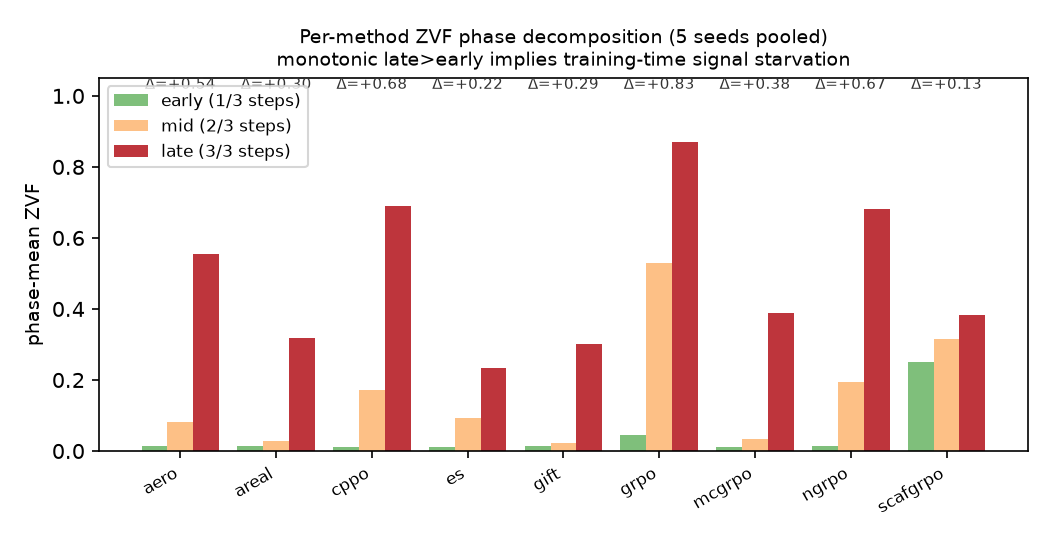
\includegraphics[width=0.85\linewidth]{figures/zvf_dynamics_phase.png}
\caption{Per-method phase-decomposed ZVF, 5 seeds pooled. Red bars
(late-phase) dominate green (early-phase) in every method. Numerical
$\Delta = \bar z_l - \bar z_e$ above each method. GRPO's late bar
reaches $0.87$, an unmistakable signal-starvation plateau.}
\label{fig:zvf-dynamics-phase}
\end{figure}

\begin{figure}[htbp]
\centering
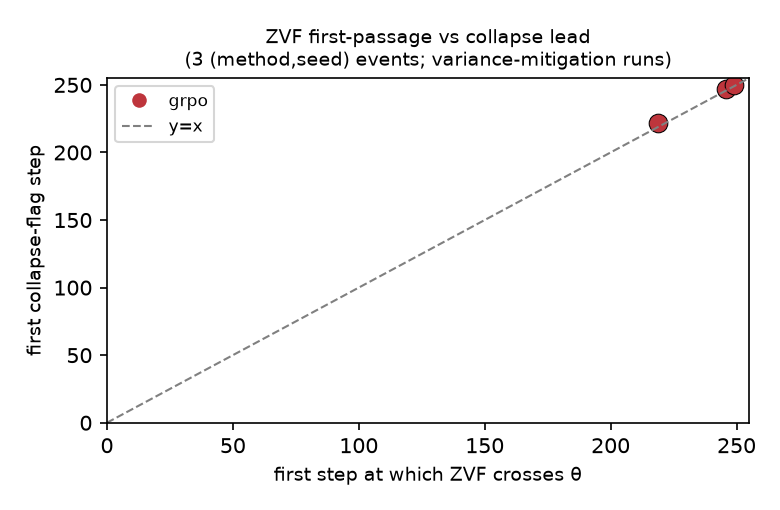
\includegraphics[width=0.75\linewidth]{figures/zvf_dynamics_leadtime.png}
\caption{First-passage step $\tau(\theta; z)$ vs.\ first collapse-flag
step $t_{\text{collapse}}$ for the 3 (method, seed) collapse events
we register. Lines parallel to $y=x$ indicate a 1-3 step gap between
threshold-crossing and collapse-flag; the gap is too short to
prescribe an early-warning intervention on this corpus, so the
operational diagnostic remains the late-phase mean ZVF rather than
the lead time.}
\label{fig:zvf-dynamics-leadtime}
\end{figure}
